\chapter{Estat de l'art}
\label{cap:estat-de-l-art}

Aquest capítol té per objectiu resumir i ordenar de forma estructurada la
recerca inicial que s'ha fet per a aquest projecte. Només es posarà èmfasi en
les parts rellevants per el projecte, però sempre s'inclourà alguna referència
per a complementar o ampliar algun concepte.

\section{\acro{Usb}}

Sent la connexió \acro{usb} un dels objectius més cèntrics d'aquest treball de
fi de grau, s'ha iniciat la recerca aquest cantó. No només s'ha escollit usar
aquest estàndard per la seva compatibilitat
i facilitats que proporciona a l'usuari, sinó que també hi havia un interès
personal en entendre aquest protocol.

El \acro{usb}, que significa \est{Universal Serial Bus} en anglès, és un
estàndard de comunicació que permet la connexió, intercanvi i transferència de
dades entre dispositius electrònics com ara ordinadors, telèfons mòbils, i
impressores. Aquesta tecnologia utilitza uns connectors estàndards que son
àmpliament reconeguts per la seva facilitat d'ús i versatilitat en una àmplia
gamma d'aplicacions. Els dispositius USB poden transmetre dades a diferents
velocitats, des de velocitats molt baixes fins a velocitats molt altes,
i són compatibles amb una gran varietat de sistemes operatius i plataformes
de hardware \cite{Axelson2015USB}.

\subsection{Arquitectura}
% Explicar mestre-esclau

\subsection{Versions}
% Explicar USB3

\subsection{Aspectes físics}

% Mida cables, extension cables

L'estàndard \acro{usb} disposa de diferents connectors. Es poden distingir en
3 grans grups: A, B i C:

\begin{figure}[ht]
    \centering
    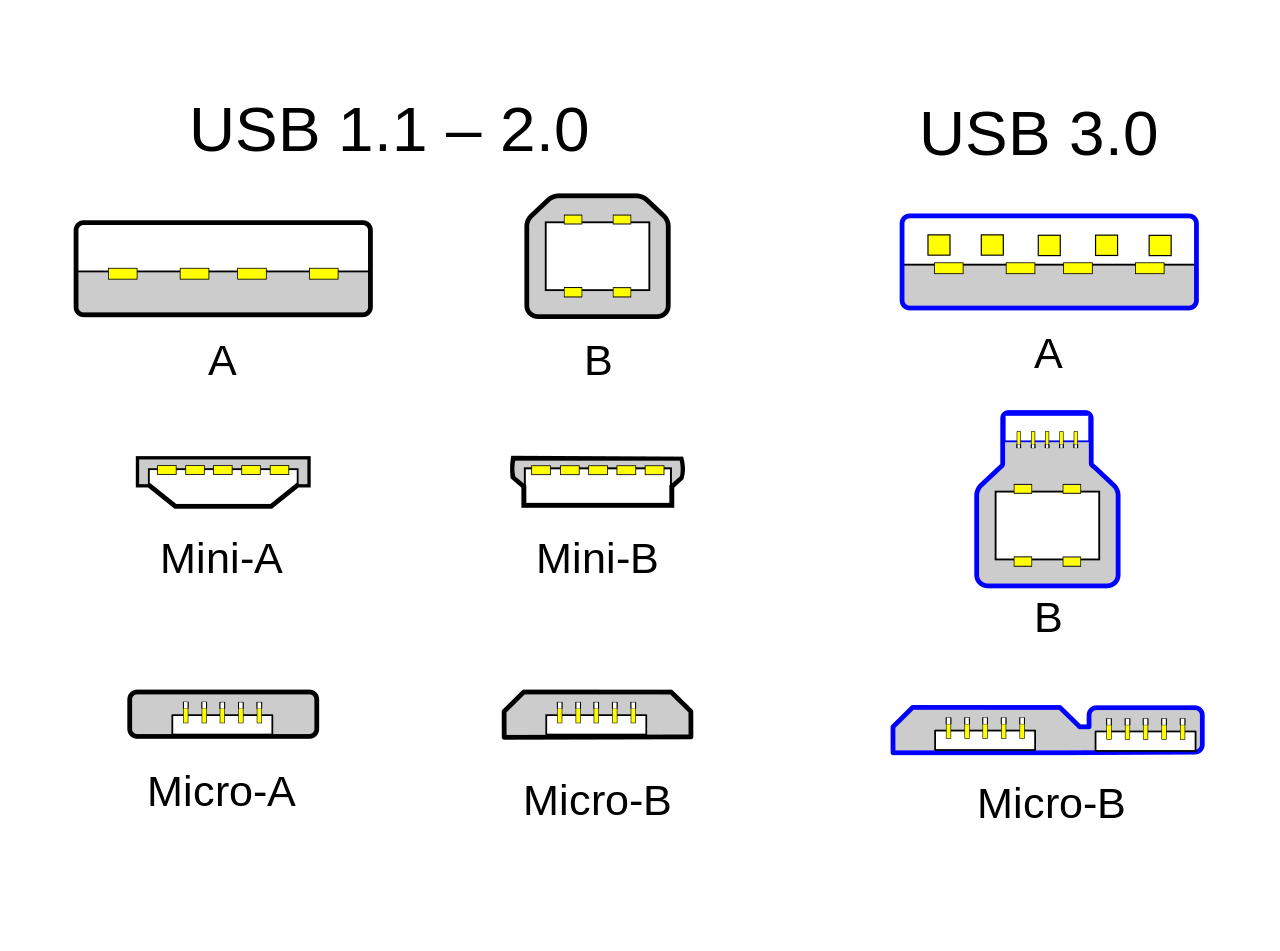
\includegraphics[width=0.6\textwidth]{images/usb_connectors.png}
    \caption{Connectors USB de tipus A i B. \cite{Contributors2024USB}}
    \label{fig:usb_connectors}
\end{figure}

\begin{itemize}
    \item Els connectors de tiups A son els que es connecten al dispositiu
    que actuarà com a mestre. Existeixen les variants \est{micro} i \est{mini},
    com es pot observar a la Figura \ref{fig:usb_connectors}, tot i que aquestes
    so son gaire populars. Amb l'aparició de l'estàndard \acro{usb3}, es van
    dissenyar nous connectors que fóssin compatibles amb els dels estàndards
    anteriors.
    \item Els connectors de tipus B son els que es connecten a l'esclau. Aquests
    també tenen les variants \est{micro} i \est{mini}, molt utilitzades
    en l'electrònica domèstica. També es va crear nous connectors de tipus B
    per a poder acollir l'estàndard \acro{usb3}.
    \item Finalment, els connectors de tipus C no tenen una jerarquia definida:
    serveixen per a dispositius que poden ser mestres o esclaus en diferents
    moments donats. La decisió de qui actua de mestre es pacta just a l'inici
    de la connexió, mitjançant un protocol específic \cite{Axelson2015USB}.
    Aquest connector, a diferència de la reta, és reversible: es pot connectar
    en les dues orientacions possibles. Es pot veure l'aspecte del connector
    a la Figura \ref{fig:usb_connectors_c}.
\end{itemize}

\begin{figure}[ht]
    \centering
    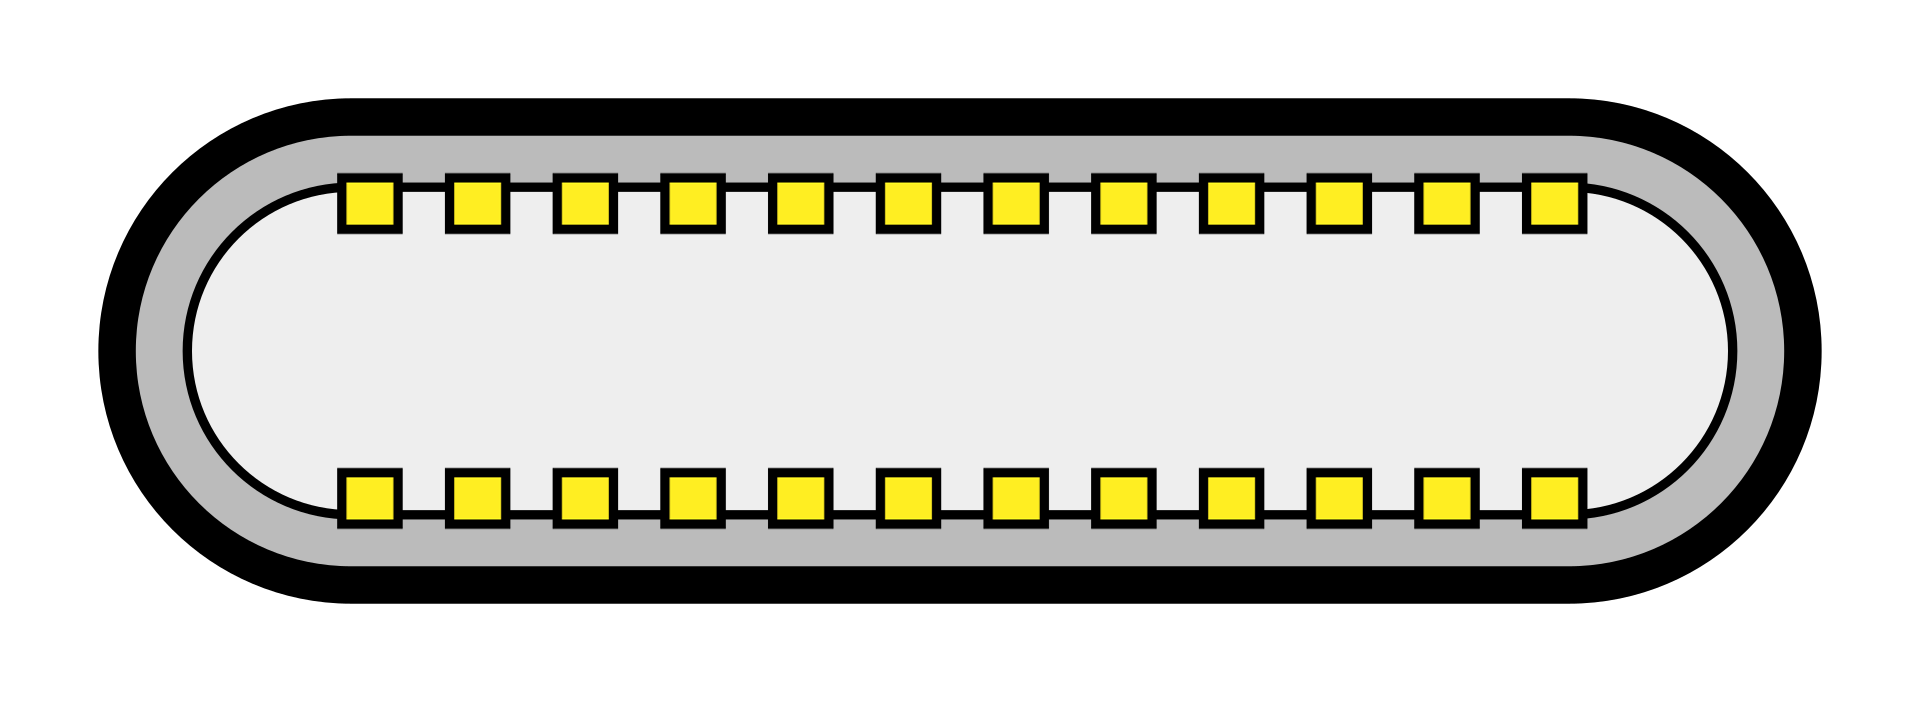
\includegraphics[width=0.3\textwidth]{images/usb_c.png}
    \caption{Connector USB de tipus C. \cite{Contributors2024USB}}
    \label{fig:usb_connectors_c}
\end{figure}

Així doncs, gairebé la totalitat de cables \acro{usb} seran de tipus A a tipus
B, utilitzant qualsevol format de mida. El tipus C, al ser bidireccional, pot
substituir el tipus A o el tipus B en els cables mencionats anteriorment.
Quan un cable només té un connector de tipus C en un cantó, no s'ha de pactar
la jerarquia de mestre-esclau, ja que ve definida pel tipus de connector a
l'altra banda del cable. Evidentment, també hi pot haver cables de tipus C a
tipus C.

Tanmateix, a l'any 2022 el Consell de la Unió Europea va aprovar una llei
que obliga un seguit de dispositius electrònics a utilitzar el connector
\acro{usb-c} enlloc d'altres estàndards \cite{Council2022Common}. Segons la
nota de premsa, el motiu d'aquesta llei és per a evitar més deixalla electrònica
per culpa de tenir diferents dispositius amb diferents connectors, així com
facilitar l'ús de les tecnologies als consumidors. Aquesta llei
es començarà a aplicar a finals de l'any 2024, i afectarà dispositius mòbils, 
alguns portàtils, tauletes, teclats i ratolins ina\l.làmbrics, entre
d'altres.

Sent el dispositu que es vol crear en aquest projecte un perifèric de
l'ordinador, la llei citada no l'afectaria. Tanmateix, la mateixa nota de premsa
informa sobre la intenció d'extendre aquest connector a altres dispositius.
Tenint present que el dispositiu que es vol crear podria entrar fàcilment en
aquest grup de perifèrics d'ordinador, s'ha decidit utilitzar un connector de
tipus \acro{usb-c} per a assegurar-nos la seva possible comercialització dintre
de la UE.
